\iffalse
\chapter{2007}
\author{EE24BTECH11060}
\section{ph}
\fi
%\begin{enumerate}[start=18]
    \item The energy levels of a particle of mass m in a potential of the form $v\brak{x}$=$\begin{cases}\infty ,x\leq 0\\ \frac{1}{2}m\omega^2x^2,x $\textgreater$ 0    \end{cases}$ are given in terms of quantum numbers $n=0,1,2,3\dots,n$ by
    \begin{enumerate}
        \item $\brak{n+\frac{1}{2}}h \omega$
        \item $\brak{2n+\frac{1}{2}}h\omega$
        \item $\brak{2n+\frac{3}{2}}h\omega$
        \item $\brak{n+\frac{3}{2}}h\omega$
    \end{enumerate}
    \item The electromagnetic field due to a point charge must be described by lienard-weichart potentials when
    \begin{enumerate}
        \item the point charge is highly accelerated.
        \item the electric and magnetic fields are not perpendicular.
        \item the point charge is moving with velocity close to that of light.
        \item the calculation is done for the radiation zone,i.e.far away from the charge.
    \end{enumerate}
    \item The strangeness quantum number is conserved in
    \begin{enumerate}
        \item strong,weak and electromagnetic interactions.
        \item weak and electromagnetic interactions only.
        \item strong and weak interactions only.
        \item strong and electromagnetic interactions only.
    \end{enumerate}
    \item The eigenvalues and eigenvectors of the matrix $\begin{bmatrix}5 &4 \\1&2\end{bmatrix}$ are
    \begin{enumerate}
        \item $6,1$ and $\begin{bmatrix}4\\1\end{bmatrix},\begin{bmatrix} 1\\-1
        \end{bmatrix}$
        \item $2,5$ and $\begin{bmatrix}4\\1\end{bmatrix},\begin{bmatrix} 1\\-1
        \end{bmatrix}$
        \item $6,1$ and $\begin{bmatrix}1\\4\end{bmatrix},\begin{bmatrix} 1\\-1
        \end{bmatrix}$
        \item $2,5$ and $\begin{bmatrix}1\\4\end{bmatrix},\begin{bmatrix} 1\\-1
        \end{bmatrix}$
    \end{enumerate}
    \item A vector field is defined everywhere as $\mathbf{F}$=$\frac{y^2}{L}\hat{i}+z\hat{k}$.The net flux of $\mathbf{F}$ associated with a cube of side $L$,with one vector at the origin and sides along the positive $X,Y$ and $Z$ axes,is
    \begin{enumerate}
        \item $2L^3$
        \item $4L^3$
        \item $8L^3$
        \item $10L^3$\\
    \end{enumerate}
    \item $\Vec{r}$ = $x\hat{i}+y\hat{j}$,then
    \begin{enumerate}
        \item $\nabla\cdot\mathbf{r}=0$ and $\nabla \abs{\mathbf{r}}=\mathbf{r}$
        \item $\nabla\cdot\mathbf{r}=2$ and $\nabla \abs{\mathbf{r}}=\hat{r}$
        \item $\nabla\cdot\mathbf{r}=2$ and $\nabla \abs{\mathbf{r}}=\frac{\hat{r}}{r}$
        \item $\nabla\cdot\mathbf{r}=3$ and $\nabla \abs{\mathbf{r}}=\frac{\hat{r}}{r}$
    \end{enumerate}
    \item Consider a vector $\Vec{p}=
    2\hat{i}+2\hat{j}+2\hat{k}$ in the coordinate system $\brak{\hat{i},\hat{j},\hat{k}}$.The axes are rotated anti-clockwise about $Y$ axis by an angle $60\degree$.The vector $\Vec{p}$ in the rotated coordinate system $\brak{\hat{i^\prime},\hat{j^\prime},\hat{k^\prime}}$ is
    \begin{enumerate}
        \item $\brak{1+\sqrt{3}}\hat{i^\prime}+3\hat{j^\prime}+\brak{1-\sqrt{3}}\hat{k^\prime}$
        \item $\brak{1-\sqrt{3}}\hat{i^\prime}+3\hat{j^\prime}+\brak{1+\sqrt{3}}\hat{k^\prime}$
        \item $\brak{1-\sqrt{3}}\hat{i^\prime}+\brak{3+\sqrt{3}}\hat{j^\prime}+2\hat{k^\prime}$
        \item $\brak{1-\sqrt{3}}\hat{i^\prime}+\brak{3-\sqrt{3}}\hat{j^\prime}+2\hat{k^\prime}$
    \end{enumerate}
    \item the counter integral $\oint \frac{1}{z^4+a^4}dz$ is to be evaluated on a circle of radius $2a$ centered at the origin .It will have contributions only from the points
    \begin{enumerate}
        \item $\frac{1+i}{\sqrt{2}}a$ and $-\frac{1+i}{\sqrt{2}}a$
        \item $ia$ and $-ia$
        \item $ia,-ia,\frac{1-i}{\sqrt{2}}a$ and $-\frac{1-i}{\sqrt{2}}a$
        \item $\frac{1+i}{\sqrt{2}}a,-\frac{1+i}{\sqrt{2}}a,\frac{1-i}{\sqrt{2}}a$ and $-\frac{1-i}{\sqrt{2}}a$
    \end{enumerate}
    \item Inverse Laplace transform of $\frac{s+1}{s^2-4}$ is
    \begin{enumerate}
        \item $\cos{2x}+\frac{1}{2}\sin{2x}$
        \item $\cos{x}+\frac{1}{2}\sin{x}$
        \item $\cosh{x}+\frac{1}{2}\sinh{x}$
        \item $\cosh{2x}+\frac{1}{2}\sinh{2x}$
    \end{enumerate}
    \item The points,where the series solution of the Legendre differential equation $\brak{1-x^2}\frac{d^2 y}{dx^2}-2x\frac{dy}{dx}+\frac{3}{2}\brak{\frac{3}{2}+1}y=0$ will diverge, are located at
    \begin{enumerate}
        \item $0$ and $1$
        \item $0$ and $-1$
        \item $-1$ and $1$
        \item $\frac{3}{2}$ and $\frac{5}{2}$
    \end{enumerate}
    \item Solution of differential equation $x\frac{dy}{dx}+y=x^4$, with the boundary condition that $Y=1$,at $x=1$,is
    \begin{enumerate}
        \item $y=5x^4-4$
        \item $y=\frac{x^4}{5}+\frac{4x}{5}$
        \item $y=\frac{4x^4}{5}+\frac{1}{5x}$
        \item $y=\frac{x^4}{5}+\frac{4}{5x}$
    \end{enumerate}
    \item Match the following\\
\begin{minipage}[t]{0.32\textwidth}
     \textbf{Column 1}\\
     \begin{enumerate}[label=(\Alph*)]
     \item rest mass
     \item charge
     \item four-momentum
     \item electromagnetic field
 \end{enumerate}
     \end{minipage}
     \hfill
\begin{minipage}[t]{0.32\textwidth}
    \textbf{Column 2}\\
    \begin{enumerate}[label=(\alph*), start=16]
    \item timelike vector
    \item Lorentz invariant
    \item tensor of rank $2$
    \item conserved and Lorentz invariant
\end{enumerate}
\end{minipage}
    \begin{enumerate}
        \item $P-2,Q-4,R-3,S-1$
        \item $P-4,Q-2,R-1,S-3$
        \item $P-2,Q-4,R-1,S-3$
        \item $P-4,Q-2,R-3,S-1$
     \end{enumerate}
     \item The moment of inertia of a uniform sphere of radius $r$ about an axis passing through its centreis given by $\frac{2}{5}\brak{\frac{4\pi}{3}r^5\rho}$.A rigid sphere of uniform mass density $\rho$ and radius $R$ has two smaller spheres of $\frac{R}{2}$ hollowed out of it,as shown in the figure. The moment of inertia of the resulting body about the $Y$ axis is
     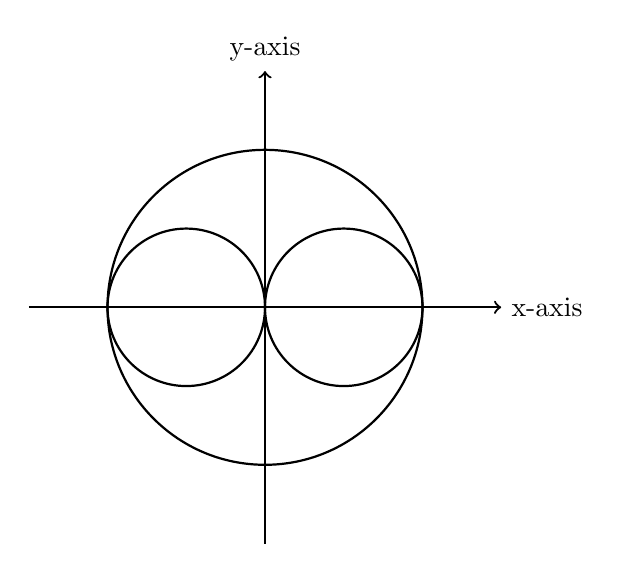
\begin{tikzpicture}

    % Define the radius of the large circle
    \def\R{2} % Radius of the large circle

    % Draw the large circle centered at the origin
    \draw[thick] (0,0) circle (\R);

    % Draw the two smaller circles
    % Each smaller circle has a radius of \R/2 and is positioned to the left and right
    \draw[thick] (-\R/2,0) circle (\R/2); % Left smaller circle
    \draw[thick] (\R/2,0) circle (\R/2);  % Right smaller circle

    % Draw the x-axis and y-axis
    \draw[->, thick] (-\R-1,0) -- (\R+1,0) node[anchor=west] {x-axis};
    \draw[->, thick] (0,-\R-1) -- (0,\R+1) node[anchor=south] {y-axis};

\end{tikzpicture}

     \begin{enumerate}
         \item $\frac{\pi \rho R^5}{4}$
         \item $\frac{5\pi \rho R^5}{12}$
         \item $\frac{7\pi \rho R^5}{12}$
         \item $\frac{3\pi \rho R^5}{4}$
     \end{enumerate}
     \item The Lagrangian of a particle of mass $m$ is $L=\frac{m}{2}\sbrak{\brak{\frac{dx}{dt}}^2+\brak{\frac{dy}{dt}}^2+\brak{\frac{dz}{dt}}^2}-\frac{V}{2}\brak{x^2+y^2}+W\sin{\omega t}$,where $V,W and \omega$ are constants.The conserved quantities are
     \begin{enumerate}
         \item energy and $z$-component of linear momentum only.
         \item  energy and $z$-component of angular
         momentum only.
         \item $z$-component of both linear and angular momenta only.
         \item energy $z$-component of both linear and angular momenta.
     \end{enumerate}
     \item Three particles of mass $m$ each situated at $x_{1}\brak{t},x_{2}\brak{t}and x_{3}\brak{t}$ respectively are connected by two springs of spring constant $k$ and un-streched length $l$.The system is free to oscillate only in one dimension along the straight line joning all the three particles.The Lagrangian of the system is
     \begin{enumerate}
         \item$ L=\frac{m}{2}\sbrak{\brak{\frac{dx_{1}}{dt}}^2+\brak{\frac{dx_{2}}{dt}}^2+\brak{\frac{dx_{3}}{dt}}^2}-\frac{k}{2}\brak{x_{1}-x_{2}-l}^2+\frac{k}{2}\brak{
         x_{3}-x_{2}-l}^2$
          \item$ L=\frac{m}{2}\sbrak{\brak{\frac{dx_{1}}{dt}}^2+\brak{\frac{dx_{2}}{dt}}^2+\brak{\frac{dx_{3}}{dt}}^2}-\frac{k}{2}\brak{x_{1}-x_{3}-l}^2+\frac{k}{2}\brak{
         x_{3}-x_{2}-l}^2$
          \item$ L=\frac{m}{2}\sbrak{\brak{\frac{dx_{1}}{dt}}^2+\brak{\frac{dx_{2}}{dt}}^2+\brak{\frac{dx_{3}}{dt}}^2}-\frac{k}{2}\brak{x_{1}-x_{2}+l}^2-\frac{k}{2}\brak{
         x_{3}-x_{2}-l}^2$
         \item$ L=\frac{m}{2}\sbrak{\brak{\frac{dx_{1}}{dt}}^2+\brak{\frac{dx_{2}}{dt}}^2+\brak{\frac{dx_{3}}{dt}}^2}-\frac{k}{2}\brak{x_{1}-x_{2}-l}^2-\frac{k}{2}\brak{
         x_{3}-x_{2}-l}^2$
     \end{enumerate}
     \item The Hamiltonian of a particle is $H=\frac{p^2}{2m}+pq$,where $q$ is the generalized coordinate and $p$ is the corresponding canonical momentum.The Lagrangian is
     \begin{enumerate}
         \item $\frac{m}{2}\brak{\frac{dq}{dt}+q}^2$
         \item $\frac{m}{2}\brak{\frac{dq}{dt}-q}^2$
         \item $\frac{m}{2}\sbrak{\brak{\frac{dq}{dt}}^2+q\frac{dq}{dt}-q^2}$
         \item $\frac{m}{2}\sbrak{\brak{\frac{dq}{dt}}^2-q\frac{dq}{dt}+q^2}$
     \end{enumerate}
     \item A toroidal coil has $N$ closely-wounded turns.Assume the current through the coil to be $I$ and the toroid is filled with a magnetic material of relative permittivity $\mu_{r}$.The magnitude of magnetic induction $\Vec{B}$ is inside the toroid,at a radial distance $r$ from the axis,is given by
     \begin{enumerate}
         \item $\mu_{r}\mu_{0}NIr$
         \item $\frac{\mu_{r}\mu_{0}NI}{r}$
         \item $\frac{\mu_{r}\mu_{0}NI}{2\pi r}$
         \item $2\pi\mu_{r}\mu_{0}NIr$
     \end{enumerate}

    
%\end{enumerate}

